\documentclass{sig-alternate-05-2015}

% Do not include ISBN and DOI info
\makeatletter
\def\@copyrightspace{\relax}
\makeatother

\begin{document}
	
	\title{CS 211 project report: \\Remote access to OpenWRT}
	
	\numberofauthors{3}
	
	\author{
		\alignauthor
		Zhehao Wang \\
               \affaddr{Department of Computer Science, UCLA}\\
		\email{zhehao@cs.ucla.edu}
		% 2nd. author
		\alignauthor
		Haitao Zhang \\
               \affaddr{Department of Computer Science, UCLA}\\
		\email{haitao@cs.ucla.edu}
		% 3rd. author
		\alignauthor 
		Jeffrey Chen\\
               \affaddr{Department of Computer Science, UCLA}\\
		\email{jc4556@g.ucla.edu}
	}
	
	\maketitle
	\section{Guideline}

	abstract; 
	introduction; 
	background;
	design; 
	implementation; 
	evaluation/demo; 
	discussions; 
	related work; 
	conclusion and future work.

	\section{Abstract}
	\section{Introduction}
	
	OpenWRT is a free, open-source, Linux-kernel based operating system (OS) for network-routing embedded systems. This OS is notable for being able to run on various types of devices and for simplifying cross-platform building of OpenWRT software packages, including fixes for devices no longer supported by the devices' manufacturers. OpenWRT receives regular updates, and allows basic router configuration, and installation of features through a package repository.
	
	OpenWRT can be configured using a SSH command-line interface or a pre-packaged LuCI web interface. The SSH command-line interface is more suitable to professional and developer users, while a web interface is more friendly to common users, providing access to basic OpenWRT functions. However, SSH is tedious on a mobile device, because the user must perform all configurations via text modifications, and data and results cannot be interpreted in visual graphics. On the other hand, OpenWRT's existing remote access web interface is made for desktop web browsers, and not smart devices. On mobile smart devices, the in-browser interface is not scaled to the dimensions of the device's screen nor is it touch-friendly, hampering user comprehension and control of the interface. Additionally, depending on the device, loss of connection or suspension of the browser to another application can force renewal of the session or prevent retrieval of network information, causing issues for presenting real-time data and visualizations.
	
	A native smart device application is more distribution-friendly for smart devices and can be designed on smart devices to be more user-friendly and streamlined to OpenWRT uses. Therefore, this project seeks to create a lightweight, easy-to-use generic Android application available for products running OpenWRT.
	
	\section{Background}
	
	\subsection{What is OpenWRT}
	OpenWRT \cite{fainelli2008OpenWRT, kim2014implementation} is a Busybox/Linux based embedded platform which is developed following GPL license. It minimizes its own functions so that it fits for lots of memory constrained devices. Specifically, it builds the appropriate toolchain for devices, compiles appropriate kernel with patched and options, and provides software as IPKG packages.
	
	\subsection{OpenWRT System Structure}
	OpenWRT System Structure covers four aspects: directory structure, packages and external repositories, toolchain, and software architecture.
	
	There are four key directories in the base: tools, toolchain, package and target.
	Tools and toolchain refer to common tools which will be used to build the firmware image, the compiler, and the C library.
	
	In OpenWRT, almost all the packages are .ipk files. Users can choose what packages to install and what packages to uninstall based on their specific needs. Packages are either part of the main trunk or maintained out of the main trunk. For the second case, packages can be maintained by the package feeds system.
	
	To compile the program for a particular architecture, the OpenWRT system will automatically create the toolchain during the cross-compilation process, simplifying the development tasks. However, if the toolchain needs to be created manually, OpenWRT also provides an easy way to configure the arguments.
	
	Figure \ref{OpenWRT:stack} shows the software stack of OpenWRT. We can see that the common embedded Linux tools such as uClibc, busybox, shell interpreter are used by OpenWRT.
	
	\begin{figure}
		\centering
		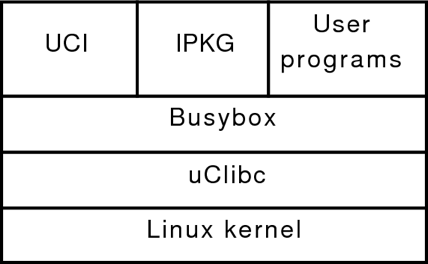
\includegraphics[width=0.4\textwidth]{stack.png}
		\caption{the software stack of OpenWRT}
		\label{OpenWRT:stack}
	\end{figure}
	
	\subsection{How to Develop With OpenWRT}
	
	It is easy to port software to OpenWRT. Various fetching methods such as GIT, Subversion, CVS, HTTP, local source can be used to download package source. In a typical package directory, there should always be a \verb|package/<name>/Makefile|. After running ``make menuconfig'', the new package will show up in the menu; and after running ``make'', the new package will be built.
	
	\subsection{Web-based Access to OpenWRT}
	In the OpenWRT system, some important features are provided: a built-in web server with CGI support, an SSH server and a package management tool. We can make use of these existing tools to build our Android application.
	
	Apart from the basic tools, OpenWRT also supports LuCI \cite{LuCI}, which is a browser-based tool to remotely configure the OpenWRT system. Specifically, it provides status visualization functions, system administration functions and network configurations. We would provide similar functions in our Android application.
	
	Another useful reference is the Netgear \cite{netgear} mobile application, which designs nice UIs that we can borrow ideas from. We need also to design the web-based access application UIs based on their work.
	
	\section{Design and implementation \\ roadmap}
	
	Based on the functional modules of LuCI, we will design the functional components of the Android application, which are organized into three major categories:
	
	\begin{itemize}
		
		\item
		\textbf{Network configuration} covers common functionalities in configuration tools that often come with commercial APs. These configurations include, but may not be limited to, managing network interfaces, DHCP and DNS settings, static routes, and firewall.
		
		\item
		\textbf{System configuration} provides an interface to customize the OpenWRT box. Common adminstration functions include: system and user configuration (setting device adminstrator password, creating system backup image and restoring system from backup image, generating user SSH keys, etc), software management (installing and configuring software packages) and task management (managing scheduled task and startup task). If the time allows, an in-application command line tool can be implemented for advanced users to execute console commands from the application to further customize the OpenWRT box.
		
		\item
		\textbf{Status/Statistics visualization} offers a mobile-phone friendly view of the system status (firmware and kernel version, uptime, current time; CPU and memory usage, currently running processes, system and kernel log) and network-related status (interface, route, firewall status, etc). The visualization component can provide real-time graphs of system load and traffic statistics, such as historical system memory usage, network traffic per interface and traffic per transport layer connection.
		
	\end{itemize}
	
	The design and implementation effort will be organized by the three function categories, with approximately one and a half weeks dedicated to each.
	
	\subsection{Graphical User Interface}
	The goal of the graphical user interface design was to simplify the user interface on a smartphone. To that end, the limitations of the LuCI web interface were studied to provide design guidelines. The first issue analyzed was that LuCI had an issue in its navigation on smartphones. To navigate through the application categories, the user needed to select a category in the navigation menu, then select a subcategory from the dropdown menu. Additionally, changing subcategories within the same category still required selecting the overarching category again. Therefore, a design goal of the application would be to maintain the current category and simply swap subcategories.
	
	Another LuCI WebView issue was that unsaved changes would be tracked in a session until committed. Tracking unsaved changes on a web browser can result in session complications, depending on browser settings for caching. Furthermore, the WebView relied on in-browser scripting to provide functional elements, which is a dependency that can be optimized. Therefore another aspect of our design was to make all actions atomic and contained to the screen they are accessed on, to avoid carrying changes. To make all actions atomic, all functional elements in the original WebView would be rebuilt natively in Android.
	
	Based on the LuCI framework, the designed Android application's user interface screens consisted of a login screen, then three major categories: status, network, and system. Each category then presented a subnavigation menu that persisted until another major category was selected, allowing users to move more freely within same category.
	
	Each separate screen in the subcategories of the major categories was designed to maintain discrete actions and information. Rather than having multiple configuration forms and submission buttons in the same screen, the screen would be limited to at most one form each, with other forms being accessible on a new screen that is linked to by a list on the current screen.

	\subsection{Application specific traffic statistics}

One of our goals in this project is to identify and provide statistics for traffic belonging to specific user applications, for example, identifying how much incoming and outgoing traffic's related with the Youtube application, and knowing which host behind this OpenWRT box is generating these traffic. To achieve this goal, we considered the following design alternatives:

\begin{itemize}

\item Install a service on each user device, which monitors application network usage information from the operating system and reports the monitored statistics to a service on the OpenWRT box. This approach can likely generate more accurate results and provide each specific application's statistics, however, it requires that each user device voluntarily run this service, which is not ideal for our goal: this service should not require additional actions from user devices, and the OpenWRT box should be able to collect statistics with or without end user cooperation.

\item Capture the traffic on the OpenWRT box, and run per-packet analysis. The following information from packet header or payload could be helpful:

  \begin{itemize}

  \item Source and destination IP addresses. Popular service providers, such as Google and Facebook, own large chunks of IP addresses, and certain destination IP address ranges may correspond to servers for a specific application. By collecting such information and building a  mapping from destination IP address to an application's backend services, we can infer the user application that's generating this traffic. The problem with this approach is that this mapping takes time to build, and it's hard for this mapping to change dynamically, especially considering the fact that many popular services are using CDNs.

  \item Source and destination port number. Certain services can be identified by IANA's port number allocation \cite{PortAssignment}, and this information is easily retrievable from the Internet. The problem with this approach, is that the amount of applications that can be identified purely by port number is very limited, for example, the Youtube app and Facebook app on Android both go through port 443 (TLS).

  \item Application layer payload. Decoding application payload and trying to find characteristic plain text is another way to identify which application the packet belongs to. This approach is promising, if such characteristic texts can be found and the payload's not encrypted, which is not the case for most popular applications, such as Youtube or Facebook. Packet capture of these apps on Android shows that their traffic goes on top of TLS, and packet capture of watching Youtube videos on a desktop indicate that the traffic goes on top of QUIC, which has encryption over UDP.

  \item Source and destination host names. DNS host names often give information about the service provider, even when the service provider's using CDNs. The assumption of this approach is that most servers or CDN boxes do have a DNS name that corresponds to the application backend that they run. Our initial experiments suggest that this assumption is indeed true for popular applications like Youtube and Facebook, though mapping a DNS domain to a certain service may not be straightforward. For example, Facebook app on Android talks to both *.facebook.com domain, and *.fbcdn.net (owned by the CDN provider, Akamai Technologies) domain, and Youtube app talks to both *.google.com, and *.1e100.net .

  \end{itemize} 

\end{itemize}

	\section{Implementation}
	\subsection{Graphical User Interface}
	The development of the user interface considered native Android solutions to the navigation. Typically, Android activities are single interface screens. Inside the Android activities, Android fragments can be used use to provide different tab screens. Therefore, tab navigation was implemented with Android activities for the categories, and Android fragments for the subcategories and forms.
	
	However, the implementation of the user interface reached complications. The major problem leading to complications was that in using the LuCI backend, content extraction using HTML retrieved whole WebView pages. JSON would extract smaller elements, but required specific queries, and would make code reuse difficult. Using both required parsing, and the extent of parsing needed for each category and subcategory complicated the implementation, taking more development time than available. The issue of parsing elements also complicated the implementation of buttons and other interactive objects, which needed to be re-made natively. Therefore, the graphical user interface was not completed in time.
	
	\section{Evaluation}
	
	\section{Discussions}
	
	\section{Future Work}
	
	\section{Conclusion}
	
	\section{Timeline}
	
	A rough timeline for the project is given in table \ref{table:timeline}.
	
	\begin{table}[h]
		\centering
		\caption{Project timeline}
		\label{table:timeline}
		\begin{tabular}{p{3cm}|p{5cm}} \hline
			Week No. & Task \\ \hline
			5, 6 (first half) & Implement status/statistics visualization module \\ \hline
			6 (second half), 7 & Implement network configuration module \\ \hline
			8, 9 (first half) & Implement system administration module \\ \hline
			9 (second half), 10 & Prepare final report and presentation \\
			\hline\end{tabular}
	\end{table}
	
  \bibliographystyle{abbrv}
  \bibliography{report}

\end{document}